
\exercise[(Forward vs.\ backward Gauss-Seidel)]{4.2}

\begin{enumerate}
\item The Gauss-Seidel method for the discretization of $u''(x) = f(x)$
takes the form (4.5) if we assume we are marching forwards across the grid,
for $i=1,~2,~\ldots,~m$.  We can also define a {\it backwards Gauss-Seidel
method} by setting
\eqlex{a}
u_i^{[k+1]} = \half (u_{i-1}^{[k]} + u_{i+1}^{[k+1]} - h^2 f_i), \qquad
\text{for}~ i = m,~m-1,~m-2,~\ldots,~1.
\end{equation}
Show that this is a matrix splitting method of the type described in
Section~4.2 with $M = D-U$ and $N=L$.

\item Implement this method in \verb+iter_bvp_Asplit.m+ and observe that it
converges at the same rate as forward Gauss-Siedel for this problem.

\item Modify the code so that it solves the boundary value problem
\eqlex{b}
\epsilon u''(x) = au'(x) + f(x),\qquad 0\leq x \leq 1,
\end{equation} 
with $u(0) = 0$ and $u(1) = 0$, where $a\geq 0$ and the $u'(x_i)$ term
is discretized by the one-sided approximation $(U_i - U_{i-1})/h$.
Test both forward and backward Gauss-Seidel for the resulting linear system.
With $a=1$ and $\epsilon = 0.0005$.  You should find that they behave very
differently:

\psfrag{forwardGS}{forward}
\psfrag{backwardGS}{backward}
\hfil\epsfig{file=figs/iter_bvp_advdiff.eps,width=3.5in}\hfil

Explain intuitively why sweeping in one direction works so much better than
in the other.

{\bf Hint:} Note that this equation is the steady equation for an 
advection-diffusion
PDE $u_t(x,t) + au_x(x,t) = \epsilon u_{xx}(x,t) - f(x)$.  
You might consider how the methods behave in the case $\epsilon = 0$.
\end{enumerate} 
